\chapter{Integrali Multipli}

\section{Definizione di Integrale Doppio}
Se pensiamo a una funzione $f(x,y) \ge 0$, il grafico della funzione sarà una porzione di superficie nello spazio 3D. 
L'integrale doppio ci permette di calcolarne il volume sotteso:
\[ \iint_\Omega f(x,y) \, dx dy = \text{volume della regione sottesa dal grafico} \]

\section{Come fare la suddivisione del dominio di integrazione?}
Se pensiamo di voler suddividere la nostra regione in un reticolo cartesiano, per poter scegliere un punto in questi sottodomini e calcolare la somma integrale, dobbiamo prima definire rigorosamente la misura di un insieme.

\subsection{Richieste da rispettare per l'area di integrazione}
\begin{enumerate}
    \item La misura di un rettangolo $\Delta$ definito da disuguaglianze del tipo $a \le x \le b$ e $c \le y \le d$ è:
    \[ m(\Delta) = (b-a)(d-c) \]
    
    \begin{center}
    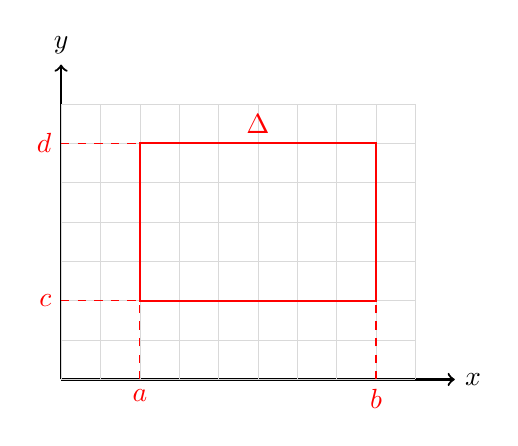
\begin{tikzpicture}
        % Assi
        \draw[->, thick] (0,0) -- (5,0) node[right] {$x$};
        \draw[->, thick] (0,0) -- (0,4) node[above] {$y$};
        % Griglia leggera
        \draw[step=0.5, gray!30, very thin] (0,0) grid (4.5,3.5);
        % Rettangolo
        \draw[red, thick] (1,1) rectangle (4,3);
        % Etichette e proiezioni
        \node[red, above] at (2.5,3) {$\Delta$};
        \draw[dashed, red] (1,0) -- (1,1);
        \node[red, below] at (1,0) {$a$};
        \draw[dashed, red] (4,0) -- (4,1);
        \node[red, below] at (4,0) {$b$};
        \draw[dashed, red] (0,1) -- (1,1);
        \node[red, left] at (0,1) {$c$};
        \draw[dashed, red] (0,3) -- (1,3);
        \node[red, left] at (0,3) {$d$};
    \end{tikzpicture}
    \end{center}

    \item Data una regione misurabile $\Omega$ suddivisa in 2 sottoregioni $\Omega_1$ e $\Omega_2$ (con intersezione interna nulla):
    \[ m(\Omega) = m(\Omega_1) + m(\Omega_2) \]

    \item Se $\Omega_1 \subseteq \Omega_2$, allora $m(\Omega_1) \le m(\Omega_2)$.
\end{enumerate}


\section{Misura interna ($m_{int}(\Omega)$)}
Data una regione $\Omega$, consideriamo la somma delle aree dei quadrati (del reticolo) contenuti interamente in $\Omega$.
Si considerano prima i quadrati di lato 1, poi di lato $1/2$, poi di lato $1/4$, e così via.
\begin{itemize}
    \item La successione delle somme delle aree interne è \textit{non decrescente}.
    \item Se la regione è limitata, la successione è \textit{limitata superiormente}. 
\end{itemize}
Pertanto, il limite esiste:
\[ m_{int}(\Omega) = \lim_{N \to \infty} m(\Omega_N^{int}) \]


\section{Misura esterna ($m_{est}(\Omega)$)}
È la somma delle aree dei quadrati che hanno intersezione (anche solo parziale) con $\Omega$.
\begin{itemize}
    \item Questa successione risulta invece \textit{non crescente} e \textit{limitata inferiormente}. Anche in questo caso il limite esiste.
\end{itemize}

\begin{center}
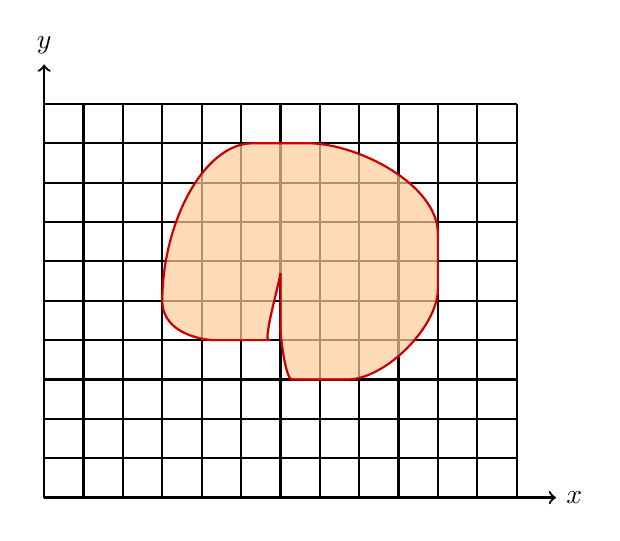
\begin{tikzpicture}[scale=0.5]
    % Griglia fitta
    \draw[step=1, black, thick] (0,0) grid (12,10);
    % Assi
    \draw[->, thick] (0,0) -- (13,0) node[right] {$x$};
    \draw[->, thick] (0,0) -- (0,11) node[above] {$y$};
    % Dominio irregolare
    \filldraw[fill=orange!40, draw=red!80!black, thick, rounded corners=10pt, fill opacity=0.7]
        (3,5) to[out=90,in=180] (6,9) to[out=0,in=90] (10,6) 
        to[out=-90,in=0] (7,3) to[out=180,in=-90] (6,5) 
        to[out=90,in=0] (5,4) to[out=180,in=-90] (3,5);
\end{tikzpicture}
\end{center}

\section{Definizione di Insieme Misurabile}
Si dice che una regione $\Omega \subset \mathbb{R}^2$ è \textbf{misurabile} (o quadrabile) se la sua misura interna coincide con quella esterna:
\[ m_{int}(\Omega) = m_{est}(\Omega) \]

\subsection{Condizione necessaria e sufficiente}
Affinché un insieme limitato sia misurabile, è necessario e sufficiente che la misura esterna della sua \textit{frontiera} sia nulla.

Questo porta alla misurabilità di una qualsiasi regione del piano che abbia come frontiera una curva regolare .

\subsection{Diametro di un insieme}
Si dice diametro di un insieme $\Omega \subset \mathbb{R}^2$ l'estremo superiore fra le distanze di tutte le possibili coppie di punti appartenenti all'insieme.

\begin{center}
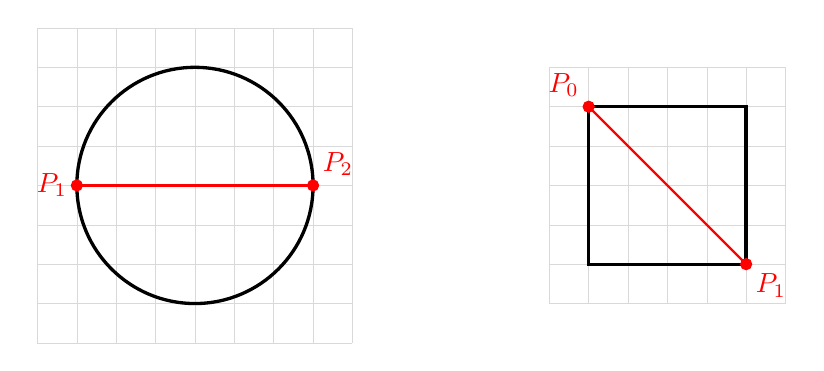
\begin{tikzpicture}
    % Cerchio
    \begin{scope}[shift={(0,0)}]
        \draw[step=0.5, gray!30, very thin] (-2,-2) grid (2,2);
        \draw[very thick] (0,0) circle (1.5);
        \filldraw[red] (-1.5,0) circle (2pt) node[left] {$P_1$};
        \filldraw[red] (1.5,0) circle (2pt) node[above right] {$P_2$};
        \draw[red, thick] (-1.5,0) -- (1.5,0);
    \end{scope}

    % Quadrato
    \begin{scope}[shift={(6,0)}]
        \draw[step=0.5, gray!30, very thin] (-1.5,-1.5) grid (1.5,1.5);
        \draw[very thick] (-1,-1) rectangle (1,1);
        \filldraw[red] (-1,1) circle (2pt) node[above left] {$P_0$};
        \filldraw[red] (1,-1) circle (2pt) node[below right] {$P_1$};
        \draw[red, thick] (-1,1) -- (1,-1);
    \end{scope}
\end{tikzpicture}
\end{center}

\section{Definizione Integrale Doppio (secondo Riemann)}
Consideriamo una regione misurabile $\Omega$ e una funzione $f: \Omega \to \mathbb{R}$. 
Data la regione, la suddividiamo in $N$ sottoregioni misurabili $\Omega_i$. In ognuna di esse scegliamo un punto arbitrario $(\xi_i)$ per costruire la \textbf{Somma integrale di Riemann}:
\[ \sum_{i=1}^N f(\xi_i) \cdot m(\Omega_i) \]

Chiamiamo $\delta$ il più grande dei diametri delle sottoregioni $\Omega_i$. Se il limite:
\[ \lim_{\delta \to 0} \sum_{i=1}^N f(\xi_i) \cdot m(\Omega_i) \]
esiste e non dipende dalle scelte della suddivisione né dalla scelta dei punti $(\xi_i, \eta_i)$, allora tale limite si dice integrale doppio di $f(x,y)$ su $\Omega$ e si indica con:
\[ \iint_\Omega f(x,y) \, dx dy \]

\subsection{Proprietà degli integrali doppi}
\begin{enumerate}
    \item \textbf{Linearità:} 
    \[ \iint_\Omega [c_1 f_1(x,y) + c_2 f_2(x,y)] \, dx dy = c_1 \iint_\Omega f_1(x,y) \, dx dy + c_2 \iint_\Omega f_2(x,y) \, dx dy \]
    
    \item \textbf{Additività rispetto al dominio:} (con $\Omega = \Omega_1 \cup \Omega_2$ a intersezione interna vuota)
    \[ \iint_{\Omega} f(x,y) \, dx dy = \iint_{\Omega_1} f(x,y) \, dx dy + \iint_{\Omega_2} f(x,y) \, dx dy \]
    
    \item \textbf{Monotonia:} Se $f_1(x,y) \le f_2(x,y)$ sono integrabili su $\Omega$, allora:
    \[ \iint_\Omega f_1(x,y) \, dx dy \le \iint_\Omega f_2(x,y) \, dx dy \]

    \item \textbf{Media Integrale:} Se $f(x,y)$ è una funzione continua in un dominio $\Omega$ chiuso, limitato, connesso e misurabile, allora esiste un punto $\xi \in \Omega$ tale che:
\[ \iint_\Omega f(x,y) \, dx dy = f(\xi) \cdot m(\Omega) \]
\end{enumerate}

\section{Integrazione per iterazione (Integrali Doppi)}

L'integrazione per iterazione si basa sul Teorema di Fubini-Tonelli e permette di scomporre un integrale multiplo in una sequenza di integrali singoli annidati. A seconda di come è fatto il dominio $D$, possiamo scegliere di integrare prima rispetto a $y$ e poi rispetto a $x$, oppure viceversa.

\subsection{Caso A: Dominio normale rispetto all'asse $x$ (y-semplice)}

Un dominio $D$ è normale rispetto all'asse $x$ se la variabile $x$ varia tra due costanti reali $a$ e $b$, mentre la variabile $y$ è compresa tra due funzioni di $x$: $g_1(x)$ (bordo inferiore) e $g_2(x)$ (bordo superiore).
\[
D = \{(x,y) \in \mathbb{R}^2 : a \le x \le b, \ g_1(x) \le y \le g_2(x)\}
\]

\begin{center}
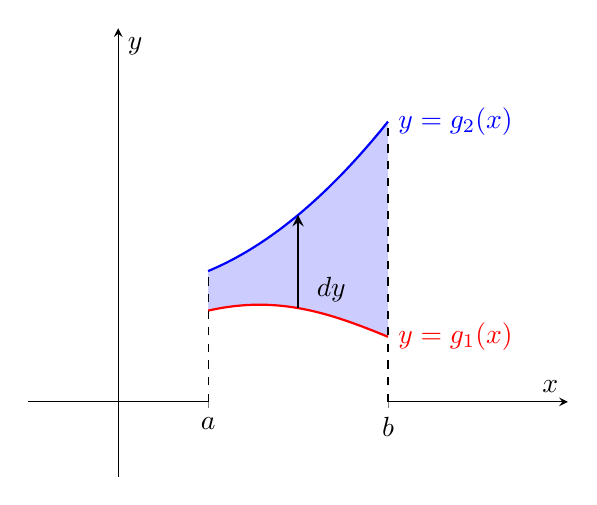
\begin{tikzpicture}
\begin{axis}[
    axis lines=middle,
    xlabel={$x$},
    ylabel={$y$},
    xmin=-0.5, xmax=4.5,
    ymin=-0.5, ymax=4.5,
    xtick={1, 3},
    xticklabels={$a$, $b$},
    ytick=\empty,
    enlargelimits=true,
    clip=false
]
% Fill the domain
\addplot[fill=blue!20, draw=none, domain=1:3, samples=50] {x^2/4 + 1.5} \closedcycle;
\addplot[fill=white, draw=none, domain=1:3, samples=50] {sin(deg(x))*0.5 + 0.8} \closedcycle;

% Draw the functions
\addplot[thick, blue, domain=1:3, samples=50] {x^2/4 + 1.5} node[above, right] {$y=g_2(x)$};
\addplot[thick, red, domain=1:3, samples=50] {sin(deg(x))*0.5 + 0.8} node[below, right] {$y=g_1(x)$};

% Draw the vertical bounds
\draw[dashed] (axis cs:1,0) -- (axis cs:1,{1/4+1.5});
\draw[dashed] (axis cs:3,0) -- (axis cs:3,{9/4+1.5});

% Draw a representative vertical slice
\draw[thick, ->, >=stealth] (axis cs:2,{sin(deg(2))*0.5 + 0.8}) -- (axis cs:2,{2^2/4 + 1.5});
\node at (axis cs:2.1, 1.5) [right] {$dy$};

\end{axis}
\end{tikzpicture}
\end{center}

In questo caso, si calcola prima l'integrale rispetto a $y$ (trattando $x$ come costante) e poi l'integrale rispetto a $x$:
\[
\iint_D f(x,y) \, dx \, dy = \int_{a}^{b} \left( \int_{g_1(x)}^{g_2(x)} f(x,y) \, dy \right) dx
\]

\textbf{Passaggi operativi:}
\begin{enumerate}
    \item \textbf{Integrale interno (verticale):} Fissato un $x$, ci muoviamo verticalmente dal bordo $g_1(x)$ al bordo $g_2(x)$ calcolando l'integrale rispetto a $y$.
    \item \textbf{Integrale esterno (orizzontale):} Integriamo la funzione risultante (che dipende solo da $x$) spostandoci orizzontalmente da $x = a$ a $x = b$.
\end{enumerate}

\subsection{Caso B: Dominio normale rispetto all'asse $y$ (x-semplice)}

Un dominio $D$ è normale rispetto all'asse $y$ se la variabile $y$ varia tra due costanti reali $c$ e $d$, mentre la variabile $x$ è compresa tra due funzioni di $y$: $h_1(y)$ (bordo sinistro) e $h_2(y)$ (bordo destro).
\[
D = \{(x,y) \in \mathbb{R}^2 : c \le y \le d, \ h_1(y) \le x \le h_2(y)\}
\]

\begin{center}
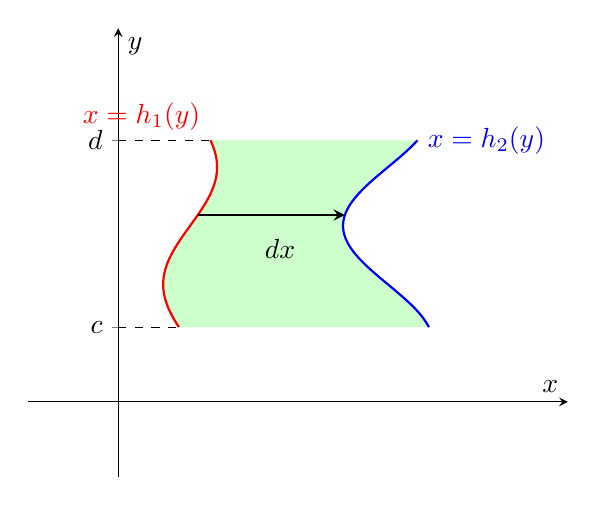
\begin{tikzpicture}
\begin{axis}[
    axis lines=middle,
    xlabel={$x$},
    ylabel={$y$},
    xmin=-0.5, xmax=4.5,
    ymin=-0.5, ymax=4.5,
    ytick={1, 3.5},
    yticklabels={$c$, $d$},
    xtick=\empty,
    enlargelimits=true,
    clip=false
]
% Fill the domain
\draw[fill=green!20, draw=none] 
    plot[domain=1:3.5, smooth] ({cos(deg(\x*2))*0.3 + 0.8}, \x) -- 
    plot[domain=3.5:1, smooth] ({sin(deg(\x*2))*0.5 + 3}, \x) -- cycle;

% Draw the functions
\addplot[thick, blue, domain=1:3.5, samples=50, variable=\t] ({sin(deg(\t*2))*0.5 + 3}, {\t}) node[right] {$x=h_2(y)$};
\addplot[thick, red, domain=1:3.5, samples=50, variable=\t] ({cos(deg(\t*2))*0.3 + 0.8}, {\t}) node[above left] {$x=h_1(y)$};

% Draw the horizontal bounds
\draw[dashed] (axis cs:0,1) -- (axis cs:{cos(deg(1*2))*0.3 + 0.8},1);
\draw[dashed] (axis cs:0,3.5) -- (axis cs:{cos(deg(3.5*2))*0.3 + 0.8},3.5);

% Draw a representative horizontal slice
\draw[thick, ->, >=stealth] (axis cs:{cos(deg(2.5*2))*0.3 + 0.8},2.5) -- (axis cs:{sin(deg(2.5*2))*0.5 + 3},2.5);
\node at (axis cs:1.8, 2.3) [below] {$dx$};

\end{axis}
\end{tikzpicture}
\end{center}

In questo caso, i ruoli si invertono: si calcola prima l'integrale rispetto a $x$ (trattando $y$ come costante) e poi l'integrale rispetto a $y$:
\[
\iint_D f(x,y) \, dx \, dy = \int_{c}^{d} \left( \int_{h_1(y)}^{h_2(y)} f(x,y) \, dx \right) dy
\]

\textbf{Passaggi operativi:}
\begin{enumerate}
    \item \textbf{Integrale interno (orizzontale):} Fissato un $y$, ci muoviamo orizzontalmente dal bordo $h_1(y)$ al bordo $h_2(y)$ calcolando l'integrale rispetto a $x$.
    \item \textbf{Integrale esterno (verticale):} Integriamo la funzione risultante (che dipende solo da $y$) spostandoci verticalmente da $y = c$ a $y = d$.
\end{enumerate}


\section{Integrazione per fili (per Integrali Tripli)}

L'integrazione per fili si usa per i domini tridimensionali $\Omega$ "semplici rispetto all'asse $z$". Il solido è limitato inferiormente da un "pavimento" $z_1(x,y)$ e superiormente da un "soffitto" $z_2(x,y)$, che si proiettano su un dominio di base $D$ nel piano $xy$.

\[
\iiint_\Omega f(x,y,z) \, dx \, dy \, dz = \iint_D \left( \int_{z_1(x,y)}^{z_2(x,y)} f(x,y,z) \, dz \right) dx \, dy
\]

\begin{center}
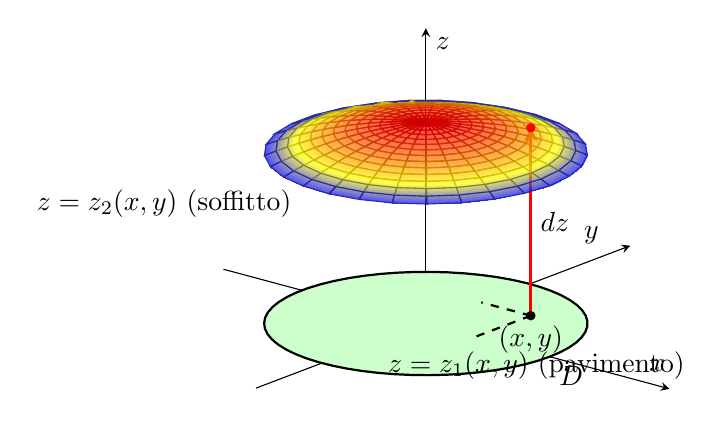
\begin{tikzpicture}
\begin{axis}[
    view={40}{30},
    width=12cm, height=9cm,
    grid=none,
    axis lines=center,
    xlabel={$x$}, ylabel={$y$}, zlabel={$z$},
    xmin=-2, xmax=2.5,
    ymin=-2, ymax=2.5,
    zmin=0, zmax=4,
    xtick=\empty, ytick=\empty, ztick=\empty,
    enlargelimits=true,
    clip=false
]

% Base domain D
\addplot3 [draw=black, fill=green!20, thick, domain=0:360, samples=60] ({1.5*cos(x)}, {1.5*sin(x)}, {0});
\node at (axis cs: 1.5, 0, 0) [below right] {$D$};

% The "filo" (thread) and points using standard pgfplots addplot3 syntax to avoid nullfont errors
\addplot3 [thick, dashed, black] coordinates {(0.6, 0.8, 0) (0.6, 0, 0)};
\addplot3 [thick, dashed, black] coordinates {(0.6, 0.8, 0) (0, 0.8, 0)};
\addplot3 [only marks, mark=*, mark size=1.5pt, black] coordinates {(0.6, 0.8, 0)};
\node at (axis cs: 0.6, 0.8, 0) [below] {$(x,y)$};

\addplot3 [very thick, red, ->, >=stealth] coordinates {(0.6, 0.8, 0) (0.6, 0.8, 2.8)};
\addplot3 [only marks, mark=*, mark size=1.5pt, red] coordinates {(0.6, 0.8, 2.8)};
\node at (axis cs: 0.6, 0.8, 1.4) [right] {$dz$};

% Surface ceiling z_2(x,y)
\addplot3 [surf, shader=faceted interp, fill opacity=0.7, domain=0:1.5, y domain=0:360, samples=15, samples y=30] 
({x*cos(y)}, {x*sin(y)}, {3 - 0.2*(x^2)});
\node at (axis cs: 0, -1.8, 2.5) [left] {$z=z_2(x,y)$ (soffitto)};
\node at (axis cs: 0.5, 1, -0.5) [below] {$z=z_1(x,y)$ (pavimento)};

\end{axis}
\end{tikzpicture}
\end{center}

\textbf{Passaggi operativi:}
\begin{enumerate}
    \item Fissato un punto $(x,y) \in D$, si percorre il "filo" verticale integrando la funzione rispetto a $z$, dalla quota inferiore $z_1(x,y)$ a quella superiore $z_2(x,y)$.
    \item Si ottiene una nuova funzione dipendente solo da $x$ e $y$.
    \item Si calcola infine l'integrale doppio di questa nuova funzione sul dominio di base $D$, utilizzando il metodo di iterazione spiegato nella sezione precedente.
\end{enumerate}